\documentclass[12pt]{article}
\usepackage[a4paper, total={6in, 10in}]{geometry}
\usepackage{graphicx}
\graphicspath{{figs/}} 


\title{Human-Humanoid Cooperation Demonstration} 
\author{Miguel Xochicale \\ 
School of Engineering \\
University of Birmingham
}
\date{November 2018}

\begin{document}
\maketitle
%\thispagestyle{empty} %No number


\begin{abstract}
Technical report for the demonstration of a human-humanoid cooperation 
activity at the Open Day at The University of Birmingham.
\end{abstract}

\section{Introduction}
For the demo, NAO, a humanoid robot \cite{gouaillier2008} has been programmed 
to move their arms from left to right in a continues way (Fig \ref{fig:nao}).




%%---------------------------------(FIGURE)-------------------------------------
\begin{figure}[!ht]
\centering
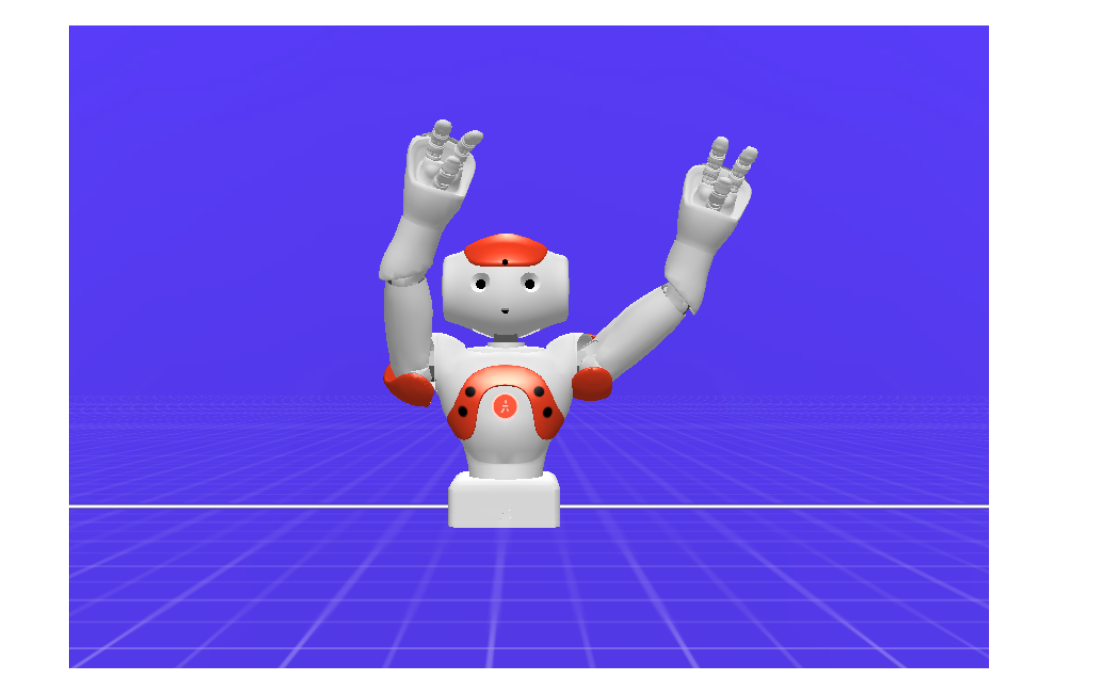
\includegraphics[width=0.5\textwidth]{nao/naoarms}
    \caption{
	{\bf Nao.}
	 Upper arm movements of NAO.
        }
\label{fig:nao}
\end{figure}
%%---------------------------------(FIGURE)------




\section{Effects of Lights with Colours}
Adquiring pictures with different light conditions
make changes of the filtered images.
It requires more investigation to tackle light 
dependencies to tackle better such problem.
It can also be raised a question regarding the consideration
of different skin colours of users when interaction with NAO.



\newpage

\bibliographystyle{apalike}
\bibliography{references/references}


\end{document}
